%%% The main file. It contains definitions of basic parameters and includes all other parts.

%% Settings for single-side (simplex) printing
% Margins: left 40mm, right 25mm, top and bottom 25mm
% (but beware, LaTeX adds 1in implicitly)
\documentclass[12pt,a4paper]{report}
\setlength\textwidth{145mm}
\setlength\textheight{247mm}
\setlength\oddsidemargin{15mm}
\setlength\evensidemargin{15mm}
\setlength\topmargin{0mm}
\setlength\headsep{0mm}
\setlength\headheight{0mm}
% \openright makes the following text appear on a right-hand page
\let\openright=\clearpage

%% Settings for two-sided (duplex) printing
% \documentclass[12pt,a4paper,twoside,openright]{report}
% \setlength\textwidth{145mm}
% \setlength\textheight{247mm}
% \setlength\oddsidemargin{14.2mm}
% \setlength\evensidemargin{0mm}
% \setlength\topmargin{0mm}
% \setlength\headsep{0mm}
% \setlength\headheight{0mm}
% \let\openright=\cleardoublepage

%% Generate PDF/A-2u
\usepackage[a-2u]{pdfx}

%% Character encoding: usually latin2, cp1250 or utf8:
\usepackage[utf8]{inputenc}

%% Prefer Latin Modern fonts
\usepackage{lmodern}

%% Further useful packages (included in most LaTeX distributions)
\usepackage{amsmath}        % extensions for typesetting of math
\usepackage{amsfonts}       % math fonts
\usepackage{amsthm}         % theorems, definitions, etc.
\usepackage{bm}             % boldface symbols (\bm)
\usepackage{graphicx}       % embedding of pictures
\usepackage{fancyvrb}       % improved verbatim environment
\usepackage{natbib}         % citation style AUTHOR (YEAR), or AUTHOR [NUMBER]
\usepackage[nottoc]{tocbibind} % makes sure that bibliography and the lists
			    % of figures/tables are included in the table
			    % of contents
\usepackage{dcolumn}        % improved alignment of table columns
\usepackage{booktabs}       % improved horizontal lines in tables
\usepackage{paralist}       % improved enumerate and itemize
\usepackage{xcolor}         % typesetting in color
\usepackage{url}
\usepackage{verbatim}
%%% Basic information on the thesis

\usepackage{acronym}
\usepackage{makecell}
\usepackage{listings}
\usepackage{enumitem}
\usepackage{bbding}
% \usepackage[nobottomtitles]{titlesec}
\newcommand\short{}

\newcommand{\emptyline}{\vspace{\baselineskip}}

\newcommand{\multilinebox}[1]{
    \begin{center}
        \framebox{
            \begin{minipage}{0.9\textwidth}
                #1
            \end{minipage}
        }
    \end{center}
}

\newcommand{\numb}[1]{
    \arabic{#1}
    \stepcounter{#1}
}

% Thesis title in English (exactly as in the formal assignment)
\def\ThesisTitle{Declarative Web Automation Toolkit}

% Author of the thesis
\def\ThesisAuthor{Jindřich Bär}

% Year when the thesis is submitted
\def\YearSubmitted{2022}

% Name of the department or institute where the work was officially assigned
% (according to the Organizational Structure of MFF UK in English,
% or a full name of a department outside MFF)
\def\Department{Department of Software Engineering}

% Is it a department (katedra), or an institute (ústav)?
\def\DeptType{Department}

% Thesis supervisor: name, surname, and titles
\def\Supervisor{RNDr. Jakub Klímek, Ph.D.}

% Supervisor's department (again according to Organizational structure of MFF)
\def\SupervisorsDepartment{Department of Software Engineering}

% Study programme and specialization
\def\StudyProgramme{Computer Science}
\def\StudyBranch{Databases and Web}

% An optional dedication: you can thank whomever you wish (your supervisor,
% consultant, a person who lent the software, etc.)
\def\Dedication{%
Dedication.
}

% Abstract (recommended length around 80-200 words; this is not a copy of your thesis assignment!)
\def\Abstract{%
The goal of this thesis is to develop a declarative toolkit for developing web automations.
Despite the great number of web automation tools and libraries on the market, it is difficult 
to find one powerful enough to meet the needs of complicated web automation use cases, yet simple enough 
to be used by untrained users. 
In this thesis, we research existing web automation tools, compare them
based on their features and ease of use, and then develop our own text format for defining web automations. 
Following this, we also develop an interpreter and a validator for this format and a design and implement 
a GUI tool for creating and editing web automations in this format. 
The user testing in the last part of the thesis describes problems the users have encountered while using
the tool. In the conclusion we try to come up with solutions to those problems and suggest ideas for further 
development.
}

% 3 to 5 keywords (recommended), each enclosed in curly braces
\def\Keywords{%
{web}, {automation}, {scraper}, {crawler}, {declarative programming}
}

%% The hyperref package for clickable links in PDF and also for storing
%% metadata to PDF (including the table of contents).
%% Most settings are pre-set by the pdfx package.
\hypersetup{unicode}
\hypersetup{breaklinks=true}

% Definitions of macros (see description inside)
%%% This file contains definitions of various useful macros and environments %%%
%%% Please add more macros here instead of cluttering other files with them. %%%

%%% Minor tweaks of style

% These macros employ a little dirty trick to convince LaTeX to typeset
% chapter headings sanely, without lots of empty space above them.
% Feel free to ignore.
\makeatletter
\def\@makechapterhead#1{
  {\parindent \z@ \raggedright \normalfont
   \Huge\bfseries \thechapter. #1
   \par\nobreak
   \vskip 20\p@
}}
\def\@makeschapterhead#1{
  {\parindent \z@ \raggedright \normalfont
   \Huge\bfseries #1
   \par\nobreak
   \vskip 20\p@
}}
\makeatother

% This macro defines a chapter, which is not numbered, but is included
% in the table of contents.
\def\chapwithtoc#1{
\chapter*{#1}
\addcontentsline{toc}{chapter}{#1}
}

% Draw black "slugs" whenever a line overflows, so that we can spot it easily.
\overfullrule=1mm

%%% Macros for definitions, theorems, claims, examples, ... (requires amsthm package)

\theoremstyle{plain}
\newtheorem{thm}{Theorem}
\newtheorem{lemma}[thm]{Lemma}
\newtheorem{claim}[thm]{Claim}

\theoremstyle{plain}
\newtheorem{defn}{Definition}

\theoremstyle{remark}
\newtheorem*{cor}{Corollary}
\newtheorem*{rem}{Remark}
\newtheorem*{example}{Example}

%%% An environment for proofs

\newenvironment{myproof}{
  \par\medskip\noindent
  \textit{Proof}.
}{
\newline
\rightline{$\qedsymbol$}
}

%%% An environment for typesetting of program code and input/output
%%% of programs. (Requires the fancyvrb package -- fancy verbatim.)

\DefineVerbatimEnvironment{code}{Verbatim}{fontsize=\small, frame=single}

%%% The field of all real and natural numbers
\newcommand{\R}{\mathbb{R}}
\newcommand{\N}{\mathbb{N}}

%%% Useful operators for statistics and probability
\DeclareMathOperator{\pr}{\textsf{P}}
\DeclareMathOperator{\E}{\textsf{E}\,}
\DeclareMathOperator{\var}{\textrm{var}}
\DeclareMathOperator{\sd}{\textrm{sd}}

%%% Transposition of a vector/matrix
\newcommand{\T}[1]{#1^\top}

%%% Various math goodies
\newcommand{\goto}{\rightarrow}
\newcommand{\gotop}{\stackrel{P}{\longrightarrow}}
\newcommand{\maon}[1]{o(n^{#1})}
\newcommand{\abs}[1]{\left|{#1}\right|}
\newcommand{\dint}{\int_0^\tau\!\!\int_0^\tau}
\newcommand{\isqr}[1]{\frac{1}{\sqrt{#1}}}

%%% Various table goodies
\newcommand{\pulrad}[1]{\raisebox{1.5ex}[0pt]{#1}}
\newcommand{\mc}[1]{\multicolumn{1}{c}{#1}}


% Title page and various mandatory informational pages
\begin{document}

\unless\ifdefined\short
	%%% Title page of the thesis and other mandatory pages

%%% Title page of the thesis

\pagestyle{empty}
\hypersetup{pageanchor=false}
\begin{center}

\centerline{\mbox{
\includegraphics[width=166mm]{./img/logo-en.pdf}}}

\vspace{-8mm}
\vfill

{\bf\Large BACHELOR THESIS}

\vfill

{\LARGE\ThesisAuthor}

\vspace{15mm}

{\LARGE\bfseries\ThesisTitle}

\vfill

\Department

\vfill

{
\centerline{\vbox{\halign{\hbox to 0.45\hsize{\hfil #}&\hskip 0.5em\parbox[t]{0.45\hsize}{\raggedright #}\cr
Supervisor of the bachelor thesis:&\Supervisor \cr
\noalign{\vspace{2mm}}
Study programme:&\StudyProgramme \cr
\noalign{\vspace{2mm}}
Study branch:&\StudyBranch \cr
}}}}

\vfill

% Zde doplňte rok
Prague \YearSubmitted

\end{center}

\newpage

%%% Here should be a bound sheet included -- a signed copy of the "bachelor
%%% thesis assignment". This assignment is NOT a part of the electronic
%%% version of the thesis. DO NOT SCAN.

%%% A page with a solemn declaration to the bachelor thesis

\openright
\hypersetup{pageanchor=true}
\pagestyle{plain}
\pagenumbering{roman}
\vglue 0pt plus 1fill

\noindent
I declare that I carried out this bachelor thesis independently, and only with the cited
sources, literature and other professional sources. It has not been used to obtain another
or the same degree.

\medskip\noindent
I understand that my work relates to the rights and obligations under the Act No.~121/2000 Sb.,
the Copyright Act, as amended, in particular the fact that the Charles
University has the right to conclude a license agreement on the use of this
work as a school work pursuant to Section 60 subsection 1 of the Copyright~Act.

\vspace{10mm}

\hbox{\hbox to 0.5\hsize{%
In \hbox to 6em{\dotfill} date \hbox to 6em{\dotfill}
\hss}\hbox to 0.5\hsize{\dotfill\quad}}
\smallskip
\hbox{\hbox to 0.5\hsize{}\hbox to 0.5\hsize{\hfil Author's signature\hfil}}

\vspace{20mm}
\newpage

%%% Dedication

\openright

\noindent
\Dedication

\newpage

%%% Mandatory information page of the thesis

\openright

\vbox to 0.5\vsize{
\setlength\parindent{0mm}
\setlength\parskip{5mm}

Title:
\ThesisTitle

Author:
\ThesisAuthor

\DeptType:
\Department

Supervisor:
\Supervisor, \SupervisorsDepartment

Abstract:
\Abstract

Keywords:
\Keywords

\vss}

\newpage

\openright
\pagestyle{plain}
\pagenumbering{arabic}
\setcounter{page}{1}


	%%% A page with an automatically generated table of contents of the bachelor thesis
\fi

\tableofcontents

%%% Each chapter is kept in a separate file
\chapter*{Introduction} \label{intro}
\addcontentsline{toc}{chapter}{Introduction}

\defcitealias{MaResFut20}{MaResFut20}
\defcitealias{Applit21}{Applit21}
\defcitealias{Chck21}{Chck21}

In the past few years, the web scraping and data extraction industry became much more prominent, as the need for data rises among all branches of science. 
The industry is expected to grow at $13.1\%$ CAGR, reaching a market value of USD $948.60$ Million \citepalias{MaResFut20}.
\par
With web browser automation also being the leading technology for UI testing and \ac{RPA} for web, the technology exceeds the data extraction needs by far.
Despite the immense size of this evergrowing industry, there is still no standardized universal format for storing automated workflows. 
Most automation developers produce executable code in general purpose programming languages, with \textit{Java}, \textit{JavaScript}, and \textit{Python} being the most prominent ones \citepalias{Applit21}.
\par
This approach poses a certain security risk, as the user of such automation needs to run untrusted code. 
It also creates a barrier to entry for beginners without the required programming knowledge. 
Furthermore, the absence of a standardized format hinders the collaboration between developers.

\section*{Thesis goals}
The goal of this thesis is to develop a human-readable, declarative format for storing and creating web automations, with an interpreter of this format and a visual editor, allowing less technical users to create and maintain automations in this format.
\par
Such format should allow for a development of resilient, reusable, and comprehensive workflow definitions. 
It should also be machine-readable, parsable and editable, ultimately leading to a simpler adoption of the format by developers of third-party software.
\par
This format should also be application-oblivious, i.e. not too oriented on automating only web-related workflows.
The definition of the format should allow developers to create interpreters for this format for handling different automation tasks, still maintaining the same syntax.
The presented workflow interpreter should then be able to parse, validate and execute the defined web-related workflows. 
It should also implement a basic programmable interface to allow other developers to use the interpreter from their own software.
\par
The workflow editor should be able to generate valid workflow files, allowing the user to create the workflow definitions without knowing the exact internal syntax of the definition format.
The editor should implement a modern, user-friendly and intuitive \ac{GUI} with a steep learning curve.
The ultimate goal of the editor is to shield the user from the programming part of the automation task completely, leaving them with a simple yet powerful graphical tool.
\chapter{Analysis} \label{analysis}

When assembling a multifunctional, reusable toolkit, it is crucial to map the exact user needs.
The following chapter analyses the user requirements and project use cases. 
It also describes different user roles and states general functional and nonfunctional requirements for the software.

% Despite the fact that this work encompasses creating a comprehensible web automation definition format, an interpreter of this format and an \ac{GUI} editor, 
% there is no point in carrying out user analysis for the format itself, since it only specifies the grammar of the definition file. 

% Therefore, the following sections conduct the analysis only for the \ac{SW} part of the work, i.e. the interpreter and the editor.

\section{User roles} \label{userroles}

In the first section of the analysis, we describe the typical users of such a toolkit.
Users may have different requirements based on their level of expertise and knowledge.
While the toolkit should be accessible and user-friendly enough to allow beginners to
create web automations with ease, it also should provide the more experienced users with 
advanced functionality required for handling specific use cases. 

For clarity, we describe only two user roles with a significant difference in skill and knowledge.
Please note that these roles are rather exemplatory and do not describe actual users the author has met.
Their main purpose is to provide a clear dichotomy between two common groups of \acl{SW} users.

\subsection{User} \label{UserUserRole}
\textit{User} has a fairly basic knowledge of using personal computers 
and web-related technologies - knowledge of e.g. \textit{CSS} or \textit{XPath} selectors is expected.
A \textit{User} wants to reach their goal without much additional knowledge and/or specialized tools.

Such a user wants to use the toolkit in the most basic way.
While they might have some experience with the technologies used in the toolkit, they generally do not want to use the toolkit programmatically and rely on the \ac{GUI} tools only.

Their automation use case is easily described, mostly as a linear sequence of well-defined, simple steps.
Some examples of such use cases might be \textit{automated data extraction} and simple \textit{\acl{RPA}}.


\subsection{Developer} \label{DevUserRole}
The \textit{Developer} user role describes an intermediate-to-expert computer specialist with deep
knowledge of computer systems, programming and web-related technologies.
This user role expects to take advantage of the advanced features of the toolkit, possibly spending some extra time learning how to use those properly.

They might not want not only to create and run automations but also to use the toolkit programmatically, 
install the toolkit components on their systems or edit parts of the toolkit. 

When creating an automation, the \textit{Developer} has more complicated use cases with possibly branching scenarios. 
Those might be more \textit{elaborate data extraction} cases, \textit{software testing}, \textit{complicated \ac{RPA}} and other.

\section{Requirements}
\label{requirements}

The following section describes functional and non-functional requirements for the toolkit project, 
based on the requirements of the user roles described in the \autoref{userroles} User roles.

For clarity, let us divide the toolkit project into individual tools serving different purposes.
As the main purposes of the toolkit are \textit{creating}, \textit{editing} and \textit{running web automations},
we can talk about the \textit{Editor} and the \textit{Runner} parts separately.

\emptyline
\subsection{Editor}

The \textit{Editor} is the part of the toolkit allowing the users to create and edit the web automations.
It should provide a user-friendly way of doing so while not restricting the more advanced users.

The ultimate goal of the \textit{Editor} is not to exhaustively support all the features of the workflow definition syntax but to provide a simple and intuitive way of creating and editing web automations.

\smallskip

\subsubsection{Functional Requirements}

\begin{enumerate}[label=\thesubsection.1.\arabic*]
    \item The \textit{Editor} must allow the user to create a valid workflow file.
    \item The \textit{Editor} must enable the user to upload a valid workflow file into the \textit{Editor}, 
    making it possible to edit this file. If the uploaded file is not a valid workflow file, the \textit{Editor}
    must reject it.
    \item The \textit{Editor} must allow the user to edit the workflow file. 
    No user-induced change to the file shall corrupt the valid file syntax.
    \item The \textit{Editor} must allow the user to export a valid workflow file. 
    This exported file must be readable by the \textit{Runner}.
    \item The \textit{Editor} must provide debugging tools for the user to check the functionality of the currently edited workflow file.
\end{enumerate}

\subsubsection{Nonfunctional requirements}

\begin{enumerate}[label=\thesubsection.2.\arabic*]
    \item The user interface of the \textit{Editor} shall be user-friendly and adhere to the best \ac{UI} practices.
    \item The \textit{Editor} shall contain workflow files for common use cases for the user to use as a boilerplate project for their own workflows
    \item The \textit{Editor} shall contain example workflow files for the user to study and to showcase the capabilities of the toolkit.
\end{enumerate}

\clearpage
\subsection{Runner}

The \textit{Runner} is the part of the toolkit providing support for executing the automations made with the \textit{Editor}.
It should provide a safe and optimized way for running the automations as well as a comprehensive user interface.

\subsubsection{Functional Requirements}

\begin{enumerate}[label=\thesubsection.1.\arabic*]
    \item The \textit{Runner} must allow the user to execute given valid automations. 
    If the provided automation is not valid, the \textit{Runner} must refuse such automation, notifying the user.
    \item If the provided automation provided to the \textit{Runner} is not valid, 
    the \textit{Runner} must provide the user with detailed information about the errors.
    \item The \textit{Runner} must allow the user to observe the automation run.
    \item The \textit{Runner} must enable the user to interrupt the automation execution at an arbitrary moment.
    \item The \textit{Runner} must provide options for debugging the automations. 
    These must expose additional information, allowing the more experienced users to facilitate the automation development.
    \item The \textit{Runner} must inform the user of any runtime errors. 
    Furthermore, the \textit{Runner} must also log all errors appropriately.
    \item The \textit{Runner} must expose a programmable interface to allow for a simple third-party adoption.
\end{enumerate}

\subsubsection{Nonfunctional requirements}

\begin{enumerate}[label=\thesubsection.2.\arabic*]
    \item The \textit{Runner} shall implement the automation execution in an optimized way.
    \item The installation of the \textit{Runner} shall be simple, allowing for quick adoption of the \acl{SW}.
\end{enumerate}
\clearpage
\section{Use case analysis}

The following section goes through multiple use cases for both the \textit{editor} and the \textit{interpreter}.
Laying out those will help with specifying the functional requirements on the \ac{SW} in the later parts of this chapter.

\subsection{Editor}

The editor is a web application facilitating the creation of the workflow definition files.
The following section sample use cases, describing the standard user flow and how the exceptions should be handled.

\newcounter{usecases}
\setcounter{usecases}{1}

\def \usecase {Use Case \numb{usecases}}

\subsubsection*{\usecase: Create a Workflow}
\begin{itemize}
    \item \textbf{Goal}: User wants to create a new empty workflow file.
    \item \textbf{Flow}: User navigates to the editor website, clicks the respective button. 
    The workflow editor interface opens with an empty workflow.
\end{itemize}

\subsubsection*{\usecase: Upload a Workflow}
\begin{itemize}
    \item \textbf{Goal}: User wants to edit an existing workflow file stored on their device. 
    \item \textbf{Flow}: User navigates to the editor website, clicks the respective button and invokes the upload form.
    The user selects the file from their device and submits it. 
    The workflow editor interface opens with an empty workflow.
    \item \textbf{Exception}: The file does not contain a valid workflow definition.
    \begin{itemize}
        \item \textbf{Exception flow}: The editor rejects such file with a comprehensive error message. The user gets navigated back to the initial site.
    \end{itemize}
\end{itemize}

\subsubsection*{\usecase: Adding a rule}
\begin{itemize}
    \item \textbf{Goal}: With a workflow file successfully opened in the editor, the user wants to add a new rule.
    \item \textbf{Flow}: User clicks the respective button. The new empty rule is added in the specified position.
\end{itemize}

\subsubsection*{\usecase: Removing a rule}
\begin{itemize}
    \item \textbf{Goal}: With a workflow file successfully open in the editor, the user wants to remove an existing rule.
    \item \textbf{Flow}: User clicks the respective button. In case the rule is not empty, the user is prompted to confirm their action.
    If this prompt message is dismissed, the rule stays in the workflow definition. In case this message is accepted, the rule is removed from the workflow definition.
\end{itemize}

\subsubsection*{\usecase: Reordering the rules}
\begin{itemize}
    \item \textbf{Goal}: The user wants to reorder the rules in an open workflow.
    \item \textbf{Flow}: User drags the rule to be repositioned. The \ac{UI} indicates the invocation drag-and-drop action.
    Dropping the dragged rule results in reordering the rules in the workflow.
\end{itemize}

\dots
\emptyline

Here follows the UML diagram specifying the relations between steps of the use cases and their relation to the end-user.

\begin{figure}[h!]
    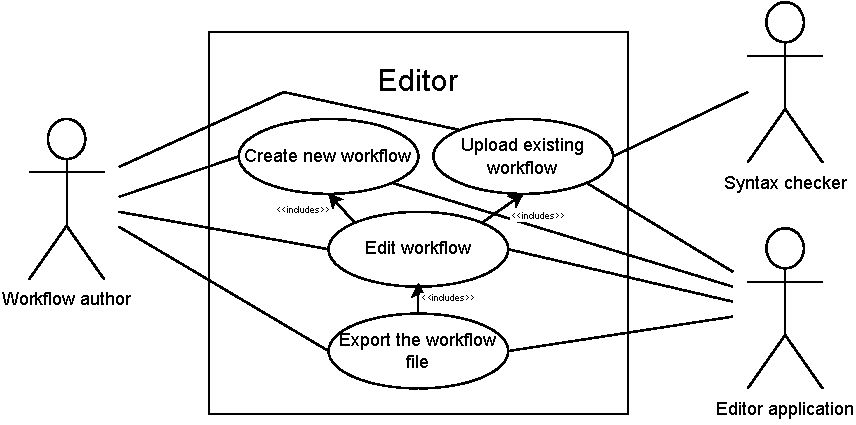
\includegraphics{./img/editorUC.pdf}
    \caption{Editor - Use Case UML diagram}
\end{figure}

% \begin{figure}[h!]
%     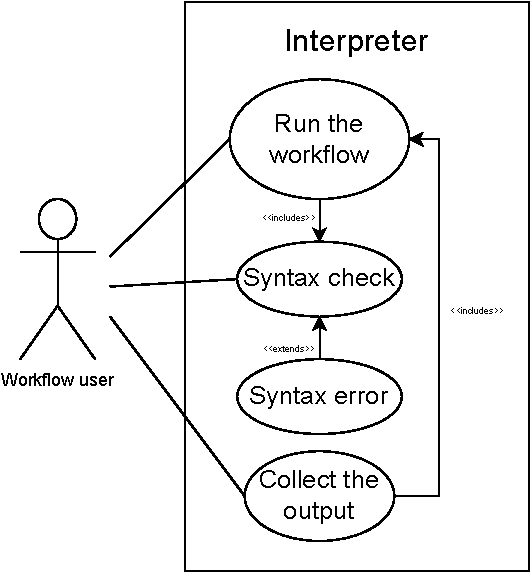
\includegraphics{./img/interpreterUC.pdf}
%     \caption{Interpreter - Use Case UML diagram}
% \end{figure}


\defcitealias{PPatch21}{PPatch21}
\defcitealias{PReadme22}{PReadme22}

\section*{Related Work}
As of now, there are already numerous solutions for automating web actions on the market. 
A majority of those uses existing web browsers and offer a programmable interface for simulating user input.

\textbf{Cypress} is a \ac{E2E} Javascript testing framework containing various assertions for \ac{QA} testing of webpages.
It supports multiple web browsers and offers its own UI and toolkit for test programming and running. 
Due to its strong orientation towards testing, it does not provide much methods for data extraction and crawling.

\textbf{Selenium WebDriver} is a fairly popular tool among web UI testers, as it offers a wide variety of methods for \ac{QA} testing.
Distributed as a multilanguage library, Selenium implements a high-level interface for controlling web browsers from code.
% Aside from regular commercial web browsers, Selenium also implements interfaces for PhantomJS and HTMLUnit, both headless scriptable browsers used as a lightweight alternative to regular browsers.

\textbf{Puppeteer} is a low-level library used for web browser automation. 
Unlike Cypress and Selenium, Puppeteer supports Chrome (or Chromium) as its only backend browser as of now (\today).

The communication with the browser is implemented via WebSockets and the DevTools Protocol, a Chromium-specific set of commands.
This allows Puppeteer to exceed Selenium both in stability and performance, sporting up to $17\%$ speedup in benchmarks \citepalias{Chck21}.

\textbf{Playwright} is another low-level library multilanguage library offering programmable ways of controlling web browser.
For browser communication, Playwright uses similiar technology as Puppeteer, unlike Puppeteer, Playwright supports multiple commercial browsers (Chromium, Firefox, Webkit as of \today).

Due to differences between browsers and partial incompatibility of protocols, Playwright is distributed with patched versions of Firefox and Webkit \citepalias{PPatch21}.
Stock versions of Chromium based browsers (Google Chrome, Microsoft Edge) are supported. \citepalias{PReadme22}

\vspace{\baselineskip}

All the aforementioned examples however require programming, which can mean a significant barrier to entry for beginners.


\chapter{Design}

This chapter describes decisions made while designing parts of the project. 
It contains separate sections for all three parts of the project, i.e. \textit{the format}, \textit{the interpreter} and \textit{the editor}.

Design decisions made here should reflect the requirements mentioned in the previous chapter.
These decisions also directly influence the implementation of the project described further.

\section{Workflow definition format}

As both the \textit{interpreter} and \textit{the editor} work directly with the files containing the workflow definitions, the first part of the project to be designed is the workflow definition format itself.

The workflow definition files should contain all the information needed to describe an arbitrary web-related workflow. 
The files in this format should also be parsable, human- and machine-readable and provide a simple yet powerful way of programming the web automations.

\subsection{Programming logic}

As the workflow definitions are computer programs of sorts, the first design decision needs to be what programming concepts will the file format implement.
To retain the steep learning curve and user-friendliness, this programming ``language'' also should not be too complicated.

The popularity of other automation tools shows that one of the simplest forms of programming is \textit{declarative programming}.
Defining the desired results rather than describing the complete control flow allows users to program the automations without being exposed to complicated programming principles.

Inspired by logic programming languages such as \textit{Prolog}, the workflow definition should contain a set of \textit{conditions} describing a possible state of the environment, connected to their respective \textit{reactions}, describing a sequence of actions to be carried out in case the condition applies.

% The similarity with \textit{Prolog} can be seen here, with the \textit{conditions} corresponding to \textit{Prolog's} fact \textit{heads} and \textit{reactions} to their respective \textit{bodies}.

\subsection{Conditions}

As stated before, the workflow definition format should allow the user to specify web environment-related conditions for running the automation steps.

Such conditions can be e.g. the browser visiting a certain \texttt{url}, the current page containing certain \texttt{selectors} or the current browser session having \texttt{cookies} set to specific values.

Moreover, the format should allow the user to combine the base conditions using \textit{boolean operators} to create more comprehensible and compact syntax.

Following through with the \textit{Prolog} comparison, the workflow definition could look something like this:

\begin{minipage}{0.95\linewidth}
\begin{verbatim}
    % X is denoting the current state of the browser
    % Y is to be unified with the next state

    nextState(X, Y) :- url(X, "https://jindrich.bar"),
                        % action to be 
                        % executed on 
                        % https://jindrich.bar
    
    nextState(X, Y) :- selector(X, "button"),
                        % action to be 
                        % executed if the current 
                        % page contains a button
    
    nextState(X, Y) :- cookies(X, "key", "value"),
                        % action to be 
                        % executed if the current 
                        % browser session has the
                        % `key` cookie for the  
                        % page set to `value`
    
    nextState(X, Y) :- url(X, "https://example.org"),
                       selector(X, "input"),
                        % action to be 
                        % executed in case of both
                        % conditions matching 
                        % (boolean AND example)

\end{verbatim}
\end{minipage}

The conditions might also provide support for advanced techniques, such as wildcards or regular expressions.
Those would be particularly useful for the URLs e.g. for targetting a specific domain, TLD etc.

\subsection{Reactions}

The workflow definition format should also allow the user to specify the actions to be carried out when the respective condition matches.

Those can be e.g. \texttt{click}, \texttt{goto}, \texttt{scrapeData} and similar. 
The actions should be chainable, allowing the user to specify a set of actions to be executed sequentially, without additional condition matching between those.

Completing the \textit{Prolog-inspired} example from the previous section, the complete workflow definition would look like this:

\begin{minipage}{0.95\linewidth}
\begin{verbatim}
    % X is denoting the current state of the browser
    % Y is to be unified with the next state

    nextState(X, Y) :- url(X, "https://jindrich.bar"),
                       goto(X, Y, "https://example.org").
    
    nextState(X, Y) :- selector(X, "button"),
                       click(X, Y, "button").
    
    nextState(X, Y) :- cookies(X, "key", "value"),
                       click(X, Y, "logout").
    
    nextState(X, Y) :- url(X, "https://example.org"),
                       selector(X, "input"),
                       fill(X, "input", "hello").

\end{verbatim}
\end{minipage}

The mock implementation of the workflow definition file in \textit{SWI-Prolog} is available as a \href{https://swish.swi-prolog.org/p/dwaim.pl}{snippet}\footnote{Available at \url{https://swish.swi-prolog.org/p/dwaim.pl}} in the \textit{Prolog} online execution environment \textit{Swish}. 

Please note that in this case, the \textit{Prolog} interpreter is actually taking role of the workflow interpreter.

\multilinebox{
    \smallskip
    \textbf{Note:} This example also shows that the new state of the browser depends only on the preceding one. 
    
    Such quality, also called \textit{memorylessness}, or \textit{Markov property}, simplifies both the interpreter design and the programming concept itself.
    It might also allow for some optimizations utilizing parallel execution. 
    \smallskip
}

\subsection{Serialization}

\defcitealias{GTrends22}{GTrends22}
\defcitealias{Medium21}{Medium21}

Finally, the workflow definition needs to be physically stored in a file. 
As it would be rather counterproductive to develop a custom file format for storing the conditions and reactions, the workflow definitions might be stored using a host meta-format.

Based on the hierarchical nature of both \textit{condition-action} pairs and possibly recursive nature of the \textit{conditions} themselves, it would be only logical to store the definitions using a hierarchical data format like \textit{JSON}, \textit{XML} or \textit{YAML}.

Comparing these formats, \textit{JSON} comes out as the most popular \citepalias{GTrends22} and most space-saving \citepalias{Medium21}. 
While the advanced features of \textit{XML} are invaluable when working with complex structured data, it is perhaps too complicated for storing well-defined workflow definitions.

With YAML taking first place, JSON is also a runner-up in human readability.
While improving the file legibility, the indentation oriented nature of YAML makes it very prone to input errors - this problem is absent in JSON because of its bracket-oriented grammar.

For the reasons mentioned, the workflow definition format will be built upon JSON - a host format providing a simple, human-readable serialization for structured schema of the definitions.

\subsubsection{}
\chapter{Implementation}

The toolkit source code is available in a public GitHub repository\footnote{\href{https://github.com/barjin/wbr/}{https://github.com/barjin/wbr/}},
along with the informal user documentation and the code and workflow file examples.
The following chapter describes the decisions made during the implementation of the toolkit.

Just like in the previous chapters, the toolkit is described in a modular fashion, following the \textit{Editor} - \textit{Runner} dichotomy.
This is also projected in the implementation, as both the editor and the runner are implemented as separate, standalone programs.
% TODO longer introduction

\section{Runner}
As stated in the \autoref{requirements} Requirements, the \textit{Runner} should be a piece of software enabling the user to run the automations created by the \textit{Editor} application.
During the implementation, only small changes were made to the initial design.

The \textit{Runner} is implemented as a \textit{Node.js} module and has been published as an \texttt{npm} package \texttt{@wbr-project/wbr-interpret}.
The user-friendly \textit{Runner} interface is a part of the \textit{Editor} application, as both tools together create a simple and easy-to-use environment for developing the web automations.

\subsection{Performance}

According to the nonfunctional requirement \textit{1.2.2.2.1}, the \textit{Runner} should implement the automation execution in an optimized way. 
While this requirement is rather vague, there are actually several ways the \textit{Runner} application tries to do so.

\subsubsection{Parallelization}

As mentioned in the \autoref{markov} Reactions, the workflow definition format is designed in such way that every step depends on the previous browser state only. 
This allows us to think of different browser tabs as of whole different environments \footnote{Only regarding the workflow execution, they still can share e.g. cookies.} 
and let the \textit{Runner} parallelize the automation between multiple tabs, possibly reducing the time required for the execution.

The \texttt{Interpreter} programmable interface allows the user to set maximum number of concurrent tabs.
Using the proper method of enqueuing links in the workflow (action \texttt{enqueueLinks}) protects the internal \textit{Runner} browser from opening too many tabs at once, which might hurt the performance.
The enqueued links are then opened as individual tabs by the \textit{Runner} with respect to the set concurrency.

In case a tab gets open e.g. as a popup window, it is not interacted with until the desired concurrency is reached.
However, accumulating multiple such tabs can still lead to performace degradation, as they still have to exist in the browser memory.

\subsubsection{Browser communication} \label{browsercom}
As mentioned in the \autoref{runnerDesign} Runner, the communication between the \textit{Interpreter} part of the \textit{Runner} and the internal web browser is facilitated using the \textit{Playwright} library.
While Playwright already provides an optimized way of communication with the browser using the \acs{CDP} protocol and alternatives, the text-based interprocess communication still poses a certain performance bottleneck.

While designing the \textit{Runner}, it was a priority to reduce the amount of calls to the \textit{Playwright} library, as pretty much any \textit{Playwright} call results in a \acs{CDP} message being sent.
During the condition matching phase of the workflow exection, the current browser state is fetched only once and the rule is then matched statically, instead of quering the browser repeatedly for the possible current URL, CSS selectors etc.

This is possible because of the simple design of the workflow definition format, allowing us to gather all the conditions statically. 
Knowing all the conditions, the full browser state can be then described by the truthiness/falsiness of those conditions, which is all that is needed for the decision making mechanism of the \textit{Interpreter} to choose the next step to take.

\subsection{Extra features}

On top of the features described in the \autoref{runnerDesign} Runner, there are some additional features implemented into the \textit{Runner} package.
While those features are tested and are available in the \verb|main| branch of the project, the other parts of the project - mainly the \textit{Editor} - typically does not provide full support.

\subsubsection{Workflow parametrization}

The \textit{Runner} module provides support for workflow parametrization. 
Any nonintegral part of the worklfow can be replaced with a special structure, for example like this:
\begin{lstlisting}[language=json]
    {
        ...
            "url": { $param: "address" },
        ...
    }
\end{lstlisting}

Before the workflow execution, the \textit{Runner} receives a dictionary of the parameters' values, replacing every \texttt{\{\$param\}} field with the declared value.
When initialized with value \texttt{\{"address" : "https://abc.xyz"\}}, the example above turns into

\begin{lstlisting}[language=json]
    {
        ...,
            "url": "https://abc.xyz",
        ...
    }
\end{lstlisting}

In case the user does not provide values for all the parameters or provides values for parameters non-existent in the workflow, the \textit{Runner} warns the user about this and does not continue with the workflow execution.

This feature can be utilized to create more universal workflow definitions, letting the end user to set certain parts of the workflow to match their use case.
The parametrized fields can be e.g. login credentials, URL of the page to run the automation on or a custom message or data to paste to the website.

\subsubsection{Automatic data extraction}

While the \textit{Runner} supports all the methods from the Playwright's \texttt{Page} class,
it also implements methods for automating data extraction from the browser.

The \texttt{scrape} method allows the user to extract data from the current page by utilizing an algorithm 
looking for the ``important'' data in the page. The user can restrict the search to a specific element subtree
by passing the selector of the root element as the only argument to this method.

The ``importance'' of the data in the page is determined using multiple heuristics, mostly by looking for 
similar-sized elements with similar content - these are believed to be the ``scrapable'' data - e.g. online store product cards, rows of a table, etc.

\subsubsection{Guided data extraction}

The \texttt{scrapeSchema} method acts as a guided counterpart of the \texttt{scrape} method.
By specifying the names of columns and their respective selectors in the only argument of this method, 
the \textit{Runner} extracts data from these selectors, and stores them in a dictionary, where the keys are the column names.

In case the selectors target multiple elements on the same page, the \textit{Runner} will group the extracted data and output multiple dictionaries.
If the numbers of the targetted elements do not match across the columns, the \textit{Runner} tries to group the data by the \acs{DOM} hierarchy in the web page, possibly leaving some output fields empty.

Here follows an example of the \texttt{scrapeSchema} method usage and the logic behind it.

\begin{figure}[!h]
    \begin{center}
        \fbox{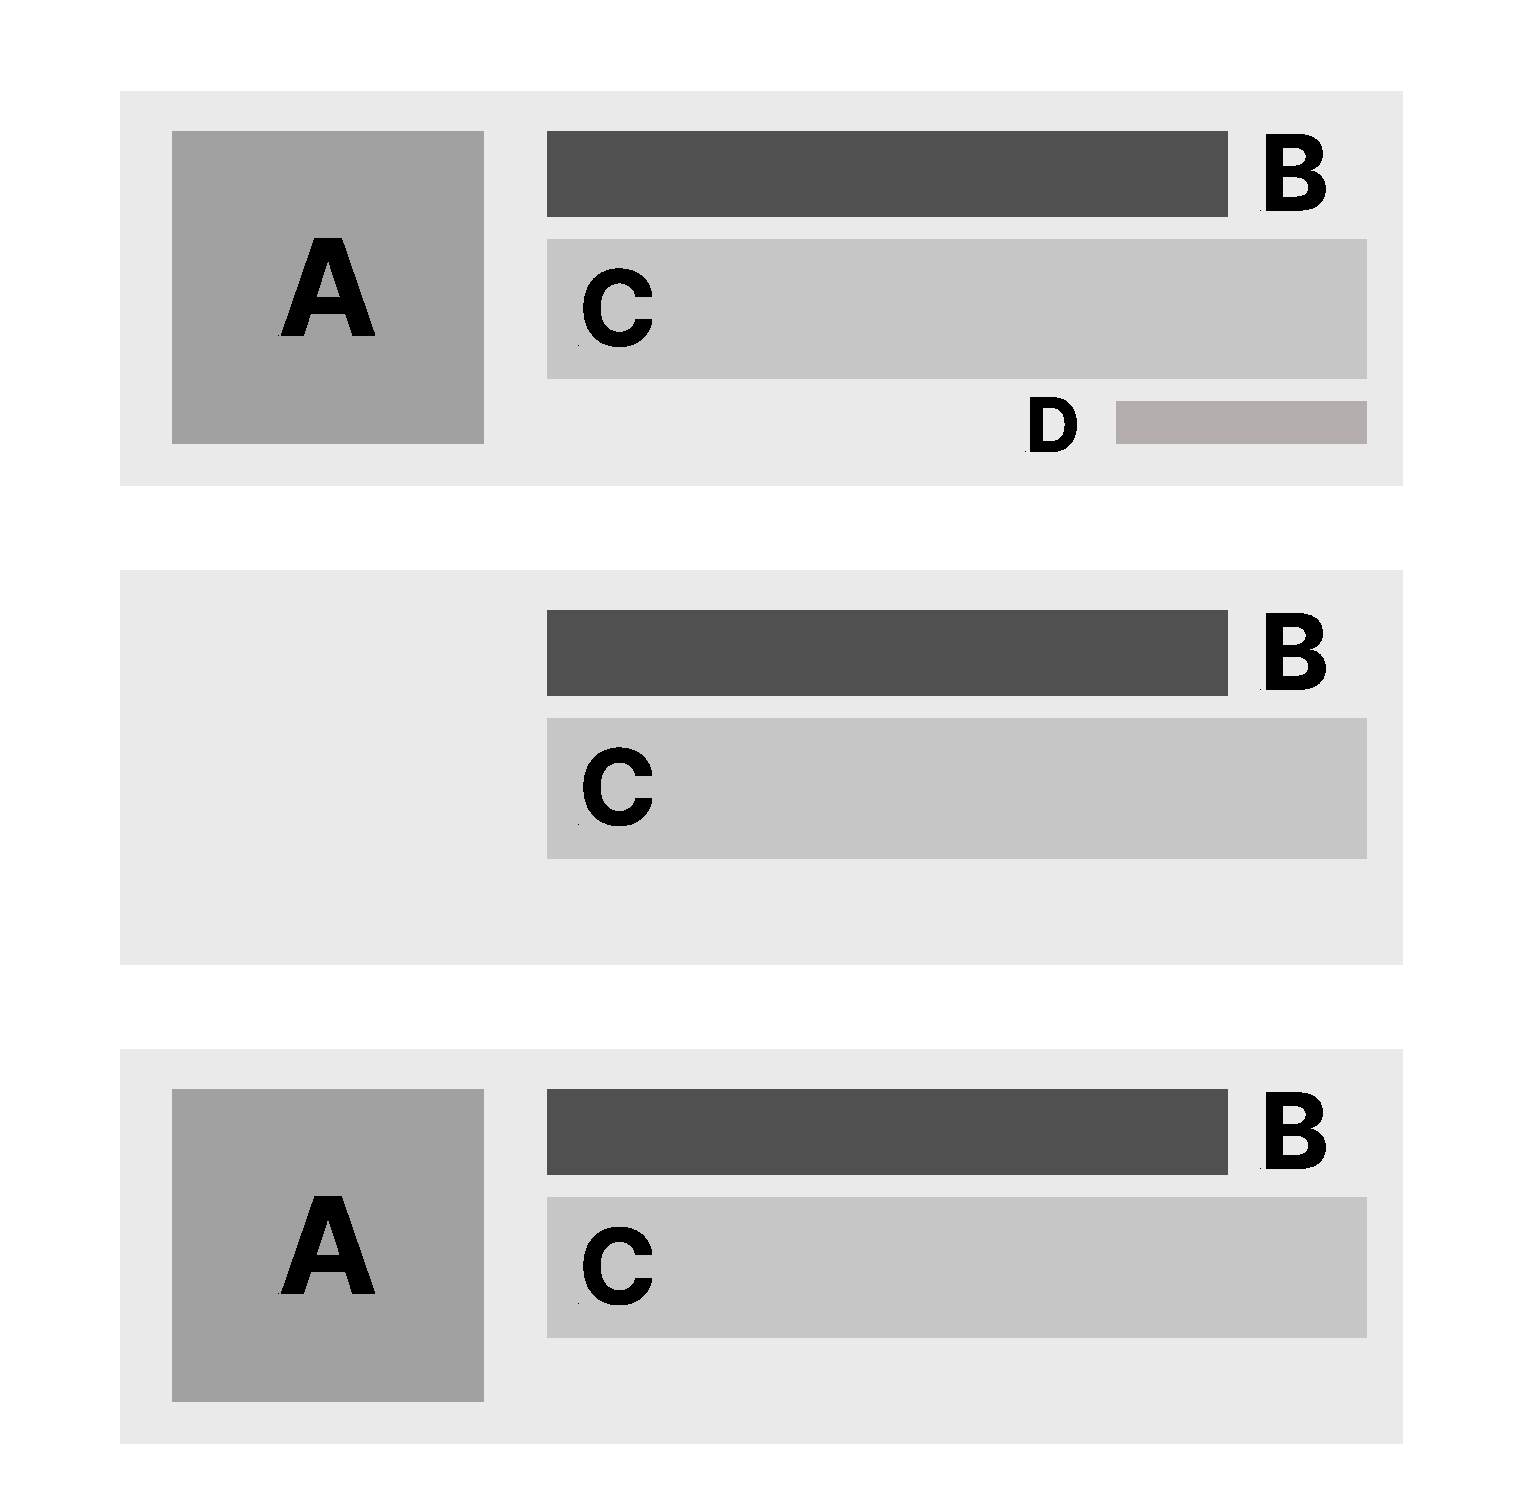
\includegraphics[width=0.4\textwidth]{./img/algos/scrapeSchema.pdf}}
    \end{center}
    \caption{Example page to be scraped}\label{scrapeSchema}
\end{figure}

The \autoref{scrapeSchema} shows an example page containing a table of user profiles. 
A user card can contain a \textit{photo of the user} (A), their \textit{name} (B), their \textit{profile description} (C) and their \textit{phone number} (D).
The letters represent the selectors for the \textit{Runner} to extract the data from.

The user provides the \texttt{scrapeSchema} method with the following schema:
    \begin{lstlisting}[language=json]
                {
                    "photo": "A",
                    "name":  "B",
                    "desc":  "C",
                    "phone": "D"
                }
    \end{lstlisting}

The \textit{Runner} extracts the data from the page. The data is stored in an array of dictionaries, where each dictionary corresponds to a user card.

\begin{lstlisting}[language=json]
[
    {
        "photo": "https://abc.xyz/img/user123.jpg",
        "name":  "John Doe",
        "desc":  "Lorem ipsum dolor sit...",
        "phone": "123-456-7890"
    },
    {
        "photo": undefined,
        "name":  "Mark Smith",
        "desc":  "Ipsum dolor amet sit...",
        "phone": undefined
    },
    {
        "photo": "https://abc.xyz/img/user234.jpg",
        "name":  "Jane Green",
        "desc":  "Sit dolor ipsum lorem...",
        "phone": undefined
    },
]
\end{lstlisting}

Note how the contents of the corresponding elements are paired, leaving the missing fields empty.
This is done by traversing the \acs{DOM} tree of the page, and grouping the elements by their common parents.

\section{Editor}
As described in the \autoref{sec:editor} \textit{Editor}, the workflow editor is implemented as a React Application.
The following section describes decisions made during the implementation of the \textit{Editor} application,
certain problems and their solutions.

% TODO add babel link
% TODO add CRA link
\subsection{React setup}
While it is possible to set up a \textit{React} application as a plain Node.js application, it is not recommended.
Handling the bundler configuration is cumbersome and requires a respectable amount of knowledge about the React toolchain.
The React's signature \acs{JSX} syntax also requires configuring a transpiler (e.g. \texttt{babel}), which adds another level of complexity.

For those reasons, the \textit{Editor} \textit{React} application has been initialized with \texttt{create-react-app}. 
This is a \ac{CLI} tool for simple initialization of \textit{React} applications.
It mainly provides the \textit{Webpack} and \textit{Babel} configuration files and bootstraps the project with a template website.

\subsubsection{Configuring Webpack polyfills}

For validating the uploaded worklflow files, the \textit{Editor} application imports the \textit{Preprocessor} class from the \textit{Interpret} module.
While both the \textit{Editor} and \textit{Interpret} module are written in \acl{TS}, there are slight differences between \textit{Node.js} and browser code.

% TODO Node.js vs browser modules citation
% TODO react-app-rewired citation
Most of those problems stem from the module resolution, as both \textit{Node.js} and browsers use slightly different approaches to module loading.
While this is covered by Webpack and Babel in most cases, importing the \textit{Interpret} module initially caused errors.

This is because since the version \texttt{5.0.0}, \textit{Webpack} no longer provides polyfills for the core \textit{Node.js} modules, such as \texttt{path} used by the \textit{Interpret} module.
The \texttt{path} module is not used by the validation feature of the \textit{Editor}, so the polyfill could be simply disabled.
However, doing so requires a manual update of the \textit{Webpack} configuration.

Since the \textit{Editor} has been created with \texttt{create-react-app}, the \textit{Webpack} configuration \texttt{webpack.conf.js} is contained in the \verb|node_modules/react-scripts| directory.
While it might be possible to modify the \texttt{webpack.conf.js} file directly, it is not recommended - the \verb|node_modules| directory is used to save all downloaded packages from NPM.
Updating the \texttt{react-scripts} package would then reset all changes made to the configuration file.
Furthermore, because of it's dynamic nature, the \verb|node_modules| directory is ommited from the \texttt{git} version control.

While the official \texttt{create-react-app} guide suggests to perform \texttt{eject}, i.e. to export the configuration files for manual maintenance, this is a borderline unsafe step. 
The \texttt{eject} script performs irreversible changes to the package structure, and forces the user to maintain the configuration and dependencies themselves from then on.

To retain the simplicity of automatic dependency management while still overriding some of the default rules, the solution now uses \texttt{react-app-rewired}.
Published as an \texttt{npm} package, \texttt{react-app-rewired} is an drop-in replacement of \texttt{create-react-app}, which lets the developer to update the configuration files, whlile still maintaining the base configuration.

\subsection{Improving the \acs{UX}}
Given the \hyperref[requirements]{nonfunctional requirements} for the \textit{Editor}, the \textit{Editor} application should adhere to the best \ac{UI}/\ac{UX} practices and provide a steep learning curve.
This is manifested multiple times in the \textit{Editor} application itself.

% TODO add react-dnd link
% TODO add react-dnd example link
\subsubsection{Drag \& Drop}
Since the main control elements in the \textit{Editor} are modular blocks, allowing the user to use drag\&drop controls e.g. for reordering the blocks seems like the superior solution in terms of UX.

The drag\&drop feature is used for reordering the blocks in the \textit{Editor} application.
While it would be possible to drag the entire blocks around the application window, it is not recommended due to UX reasons.
This is solved in the \textit{Editor} application by collapsing all the blocks when the drag\&drop action is initiated.
This helps the user to focus on the actual meaning of the reordering action, and not on the content of the blocks.

The implementation of the drag\&drop feature is based on the \texttt{react-dnd} library.
While the authors of this library offer an official example of reordering a list of block elements, the \textit{Editor} implementation is not based on this example due to the mentioned reasons.

\subsubsection{Argument type suggestions}
The \textit{Editor} application generates a workflow interpretable by the \textit{Runner} application, which is internally using the \textit{Playwright} library.
The function signatures of the workflow reaction steps depend on the \textit{Playwright} library, as most of the supported steps are mirrored from the \texttt{Page} class methods.
While the user might set the types of the arguments themselves, the \textit{Editor} application aims to provide a simple way of creating the web automations.

For this reason, the \textit{Editor} application provides a prefilled list of arguments with the correct types and matching input elements,
which correspond to the \textit{Playwright} \texttt{Page} class methods and present the correct usage of the arguments to the user.

\subsubsection{}


\chapter{Documentation}

The following chapter contains the documentation of the project. 
It is divided into several sections based on the amount of experience of the reader and the desired actions.

\defcitealias{DockerRun}{DockerRef}

\section{Administrator documentation} \label{adminDocs}

The following section contains the administrator documentation of the project.
It contains installation instructions and a short troubleshooting guide for setting up a server for the \textit{Editor} and \textit{Runner} applications. 
It also contains a list of system requirements on the server where the applications are to be deployed.

Aside from this, this section also contains installation instructions for the \textit{Runner} \texttt{npm} package, enabling the user to create software able to execute and validate the workflow definition files.

\subsection{Editor application}

% TODO: initial words

\subsubsection{Installation instructions}

The \textit{Editor} and \textit{Runner} application are both packaged in the \href{https://www.docker.com/}{Docker} image \texttt{barjin/wbr}.
This Docker image\footnote{Tag \texttt{barjin/wbr:final}, \texttt{sha256:b9e237a3ccf619f4a9b36e6584191bf}} represents a complete server setup, including all the dependencies and the \textit{Editor} and \textit{Runner} applications.
To run a Docker image, the workstation must have \textit{Docker} installed. 
Aside from meeting the \textit{Docker} system requirements, the \textit{Editor} Docker image presses no other requirements on the workstation.

The web server providing the user interface is running on port \texttt{8080} of the Docker container, which is also the only port utilized by the \textit{Editor} and \textit{Runner} applications.
On a system with \texttt{docker} installed, running the container requires only one command:

\begin{verbatim}
            docker run -p HOSTPORT:8080 -d barjin/wbr
\end{verbatim}
where \texttt{HOSTPORT} is the port number used by the \textit{Editor} and \textit{Runner} applications on the host machine.
After running this command, the user interface should be now available at \texttt{http://localhost:HOSTPORT/}.

The \texttt{-d} option instructs Docker to run the container in so-called `detached mode', which means that the container is not terminated when the command finishes. \citepalias{DockerRun}
In case the user wants to stop the container, they can use the \texttt{docker stop} command with the container ID.

In case the user never ran the \texttt{docker run} nor the \texttt{docker pull} command before, the \textit{Docker daemon} first downloads the \texttt{barjin/wbr} image from the Docker Hub.
Note that this can cause a delay of several seconds and consume a certain amount of bandwidth (ca. 200 MiB).

The Docker image can also be built from the attached Dockerfile by invoking the \texttt{docker build} command in the root folder of the project repository.

Please note that the \textit{Editor} application allows the users to run arbitrary code on the server.
This is a security risk, and the user is advised to only share their instance of \textit{Editor} server with trusted users.

\subsubsection{Build instructions}
Besides the \textit{Docker} image, all the software source files are also available in the project's GitHub repository.\footnote{Tag \texttt{v1.0}, commit hash \texttt{bf45528225e3b9fc05963d75}}

The \texttt{package.json} files for the packages \texttt{wbr-interpret}, \texttt{wbr-editor} and \texttt{wbr-cloud} contain the build instructions for the respective applications,
as well as the required dependencies.

\multilinebox{
    \textbf{Note:} \texttt{npm} is required for building the \textit{Editor} and \textit{Runner} applications.
    Before building the applications, run
    \begin{center}
    \texttt{npm run confBuildDeps}
    \end{center}
    command in the root folder of the project repository.
    This installs the correct versions of build dependencies in the correct order. 
    Running the \texttt{build} command without the dependency installation - or installing the build dependecies in a different way - can result in build errors and/or unexpected behavior.
}

The build process is managed by the \textit{Turborepo}\footnote{\url{https://turborepo.org/}} build system. 
\textit{Turborepo} allows for faster build times and less wordy build configurations by utilizing a \texttt{make}-like approach 
to the build process. It caches the built files and allows for incremental builds and faster rebuilds. 
It also constructs a dependency graph of the source packages by reading their \texttt{package.json} files, which is used to determine the order in which the packages are built.

The \texttt{turbo} build is invoked by the \texttt{npm run build} command in the root folder of the repository.
Invoking the \texttt{npm start} command in the root folder of the repository after the build starts the \textit{Editor} application server.
\chapter{Testing}

During the development phase, all parts of the project have been tested using various testing methods.
The following chapter describes the testing methodology and the nature of the individual tests.
Aside from testing the software using automated test suites, user testing was carried out on the \textit{Editor} application.

\section{Code quality}

While the code quality does not directly influence the correctness of the results, it is an important aspect of the project, as it influences readability and maintainability of the code.
Maintaining a consistent code style also speeds up the development process and reduces the risk of introducing bugs.

The \texttt{wbr-interpret} module and the \textit{Editor} application are written in \textit{TypeScript} and \textit{TSX}, respectively.
The codebase of the entire project follows the practices described in the \textit{Airbnb JavaScript Style Guide}\footnote{\href{https://airbnb.io/javascript/}{https://airbnb.io/javascript/}}, made and maintained by \textit{Airbnb, Inc.}
\textit{Airbnb Inc.} also provides a \texttt{.eslintrc} file for configuring \textit{ESLint} in accordance with the practices described in the \textit{Style Guide}.
All the code in the project is then automatically checked for conforming to the style guide using \texttt{ESLint} already during the development phase, which simplifies formatting and allows us to see potential errors right away.

The project's GitHub repository also contains an automated \textit{GitHub Actions} workflow, running the \textit{ESLint} check with every push to the repository.
This helps with catching the bad code patterns early on and prevents the need for further manual testing.

\section{Automated tests}

To ensure the elementary correctness of the project parts, the project has contained automated test suites since the early stage of development.
This helps both with code maintenance and new feature implementation, as the automated test suites ensure we do not introduce any breaking changes.

All of the tests mentioned in the following sections are also ran in the corresponding \textit{GitHub Actions} workflow. 
This ensures that the code available in the main branch of the public repository is always tested against the latest changes.

All the following tests were carried out using the \texttt{jest}\footnote{\href{https://jestjs.io/}{https://jestjs.io/}} testing framework, if not stated otherwise.

\subsection{Unit tests}

The entirety of the \texttt{wbr-interpret} package is covered with unit tests testing the individual components of the package.
Special attention is paid to the \textit{Interpreter} and \textit{Preprocessor} classes, as those are the core of the project
and contain the largest amount of complex code. 

The success of the unit tests is directly related to the code design of the module, 
since almost all methods in both classes were first written as pure functions, and only then they were converted to classes for
encapsulation and to provide a more convenient interface.

\smallskip
While it is possible to unit test components in a React application, most of the components in the \textit{Editor} application are trivial.
For this reason, there are no unit tests for the \textit{Editor} application and all the testing is carried out by \ac{E2E} tests.

\subsection{E2E tests}

Both the \textit{Editor} application and \texttt{wbr-interpret} package have been tested with \acl{E2E} tests as well.
These tests are typically longer and follow a complete user path, testing the entire application from the user's perspective.

The \texttt{wbr-interpret} package is \acl{E2E} tested for two different scenarios:
\begin{itemize}
    \item Loading, validating and executing a simple workflow.
    \item Loading, validating, initializing and executing an advanced, parametrized workflow.
\end{itemize}

Both \ac{E2E} tests are run against a local server, which is started before the tests are run.
This way we can observe the actions carried out by the \textit{Runner} even without obtaining any output data.

The \textit{Editor} application has been tested using \textit{Playwright} library to simulate the user's interaction with the application.
There are two tested scenarios:
\begin{itemize}
    \item Uploading various workflow files and seeing which one is valid. 
    \item Creating new automation, editing it, running it, seeing the results and downloading the workflow definition file.
\end{itemize}

All the automations are also run against a local server, which allows us to control the content of the webpages 
and observe the actions caused by the automation execution.

\section{User testing}

Aside from the code testing, the \textit{Editor} application has also been tested by 8 potential users of different technical backgrounds.
This was done in two parts.
First, the users were asked to use the \textit{Editor} application to create a simple automation file.
After getting accustomed to the software, the users were given a \ac{SUS} survey and were asked to rate the application's usability.

\subsection{Test scenario}

The task for the users testing the \textit{Editor} application was to create a simple web automation using the application and execute it to validate the functionality.
Such a task requires utilizing a number of \acs{UI} elements of the \textit{Editor} application, while not being too demanding or requiring much technical knowledge.

\smallskip
The created automation should be able to perform the following steps:
\begin{enumerate}
    \item Navigate to \href{https://jindrich.bar/}{https://jindrich.bar/}.
    \item Click an arbitrary link on the page.
    \item If the resulting page contains paragraphs with text, download these first, otherwise just terminate the execution.
\end{enumerate}
    
The users were provided no additional support during the task.
Out of the eight users, only three of them were able to successfully complete the task, while the others failed at various points.
The successful users were all computer specialists with a strong technical background.
While this might show a trend towards excessive technicality of the application, the sample size is not significant enough to make any conclusions.

The individual user complaints bring better insight into the why some users failed to complete the task.
The less successful users complained mostly about the complexity of the workflow definition format and
the confusing logic of the workflow interpretation.

There were no direct complaints about the application's user interface layout. 
After concluding the experiment, all of the users were instinctively able to find all the control elements when asked to perform a specific action.
All of them were also able to answer questions about the system state.

\subsection{SUS survey}
All the testers have also shared their opinions on the usability of the application via the \ac{SUS} survey.
The detailed results of the \ac{SUS} survey are included in the \hyperref[sec:sussurvey]{Attachment A.1} SUS Survey Results.
The attachment also contains additional information about the survey itself.

The average \ac{SUS} score over the ratings of the eight users is \textbf{52.5}.
This sets the \textit{Editor} application somewhere between the \textit{10th} and \textit{20th} percentile of typical \ac{SUS} evaluated systems.
While this might come off as negative result, it is still a valuable indicator of the quality of the \textit{Editor} application.

The main reasons for the low ratings the users stated were \textit{the workflow definition format being confusing} and the general unfamiliarity with debugging tools. 
While it would be easy to brush these points off as too subjective, the goal of the thesis was to create a tool that would be easy to use and intuitive for the user -
which makes all the user complaints very relevant.
\chapter{Conclusion}

The goal of this work, as stated in the \hyperref[intro]{Introduction} was to \textit{create a human-readable, declarative format for
storing and creating web automations, with an interpreter of this format and a
visual editor, allowing less technical users to create and maintain automations in
this format.}

By implementing the \textit{Editor} application and the \textit{Runner} module, this goal has been achieved in full scale.
Both parts of the project are now fully functional - in accordance with the requirements from the \autoref{requirements} Requiements - and can be used to create and edit web automations
for data extraction and process automation.
Both parts of the project have been developed in a modular fashion, which makes the further development process easier and faster.

Future work on the project includes further simplification of the \textit{Editor} application, as the current implementation does not quite fulfill the user expectations.
The simple format design could allow for automatic generation of the workflow definition files, allowing the users to create the resilient web automations by e.g. recording their actions in a browser. 
The \textit{Runner} module could also be updated with more advanced features, better support for automated data extraction or support for crawling the web.

\chapter*{Conclusion}
\addcontentsline{toc}{chapter}{Conclusion}


%%% Bibliography
%%% Bibliography (literature used as a source)
%%%
%%% We employ bibTeX to construct the bibliography. It processes
%%% citations in the text (e.g., the \cite{...} macro) and looks up
%%% relevant entries in the bibliography.bib file.
%%%
%%% The \bibliographystyle command selects, which style will be used
%%% for references from the text. The argument in curly brackets is
%%% the name of the corresponding style file (*.bst). Both styles
%%% mentioned in this template are included in LaTeX distributions.

\bibliographystyle{plainnat}    %% Author (year)
% \bibliographystyle{unsrt}     %% [number]

\renewcommand{\bibname}{Bibliography}

%%% Generate the bibliography. Beware that if you cited no works,
%%% the empty list will be omitted completely.

\bibliography{bibliography}

%%% If case you prefer to write the bibliography manually (without bibTeX),
%%% you can use the following. Please follow the ISO 690 standard and
%%% citation conventions of your field of research.

% \begin{thebibliography}{99}
%
% \bibitem{lamport94}
%   {\sc Lamport,} Leslie.
%   \emph{\LaTeX: A Document Preparation System}.
%   2nd edition.
%   Massachusetts: Addison Wesley, 1994.
%   ISBN 0-201-52983-1.
%
% \end{thebibliography}


%%% Figures used in the thesis (consider if this is needed)
\listoffigures

%%% Tables used in the thesis (consider if this is needed)
%%% In mathematical theses, it could be better to move the list of tables to the beginning of the thesis.
\listoftables

%%% Abbreviations used in the thesis, if any, including their explanation
%%% In mathematical theses, it could be better to move the list of abbreviations to the beginning of the thesis.

\chapwithtoc{List of Abbreviations}

\begin{acronym}
 \acro{GUI}{graphical user interface}
 \acro{API}{application programming interface}
 \acro{CLI}{command line interface}
 \acro{RPA}{robotic process automation}
 \acro{QA}{quality assurance}
 \acro{E2E}{end-to-end}
 \acro{SW}{software}
 \acro{UX}{user experience}
 \acro{UI}{user interface}
 \acro{CDP}{Chrome DevTools Protocol}
 \acro{IDE}{integrated development environment}
 \acro{JS}{JavaScript}
 \acro{TS}{TypeScript}
 \acro{JSX}{JavaScript Extended Syntax}
 \acro{HTML}{Hypertext Markup Language}
 \acro{WYSIWYG}{\href{https://en.wiktionary.org/wiki/WYSIWYG}{What You See Is What You Get}}
 \acro{DOM}{Document Object Model}
 \acro{CORS}{cross-origin resource sharing}
 \acro{NPM}{\href{https://www.npmjs.com/}{Node Package Manager}}
 \acro{SUS}{Software Usability Scale}
\end{acronym}

%%% Attachments to the bachelor thesis, if any. Each attachment must be
%%% referred to at least once from the text of the thesis. Attachments
%%% are numbered.
%%%
%%% The printed version should preferably contain attachments, which can be
%%% read (additional tables and charts, supplementary text, examples of
%%% program output, etc.). The electronic version is more suited for attachments
%%% which will likely be used in an electronic form rather than read (program
%%% source code, data files, interactive charts, etc.). Electronic attachments
%%% should be uploaded to SIS and optionally also included in the thesis on a~CD/DVD.
%%% Allowed file formats are specified in a provision of the rector no. 72/2017.
\unless\ifdefined\short
	\appendix
	\chapter{Attachments}
	\section{SUS survey details}
	\label{sec:sussurvey}
	This Attachment contains the detailed results of the \ac{SUS} survey for the \textit{Editor} application.
	While the \ac{SUS} is somewhat standardized set of questions for evaluating the quality of software,
	the questions can be updated to match the evaluated software's needs. For completeness, the questions are included in here:
	\begin{enumerate}
		\item I think that I would like to use this application frequently.
		\item I found the application unnecessarily complex.
		\item I thought the application was easy to use.
		\item I think that I would need the support of a technical person to be able to use this application.
		\item I found the various functions in this application were well integrated.
		\item I thought there was too much inconsistency in this application.
		\item I would imagine that people would learn to use this application very quickly.
		\item I found the application very cumbersome to use.
		\item I felt very confident using the application.
		\item I needed to learn a lot of things before I could get going with this application.
	\end{enumerate}
\smallskip
	The response scale for each question is then a 5 point Likert agreement scale:
	\begin{center}
	\begin{tabular}{c | c | c | c | c}
		Strongly disagree &	Disagree & \makecell{Neither agree\\ nor disagree} & Agree & Strongly agree \\
		\hline
1 & 2 & 3 & 4 & 5 \\
	\end{tabular}
	\end{center}

	The results of the evaluees' survey are presented in the following table:
	\begin{center}
		\begin{tabular}{ c | c | c | c | c | c | c | c | c | c | c | c } 
							 & 1 & 2 & 3 & 4 & 5 & 6 & 7 & 8 & 9 & 10 & \textbf{SUS} \\
							 \hline\hline
\textbf{User 1} & \textbf{3} & \textbf{2} & \textbf{4} & \textbf{2} & \textbf{3} & \textbf{2} & \textbf{3} & \textbf{2} & \textbf{4} & \textbf{1} & \textbf{70} \\
\textbf{User 2} & \textbf{2} & \textbf{2} & \textbf{2} & \textbf{3} & \textbf{4} & \textbf{3} & \textbf{2} & \textbf{2} & \textbf{3} & \textbf{2} & \textbf{52.5} \\
\textbf{User 3} & \textbf{4} & \textbf{2} & \textbf{4} & \textbf{2} & \textbf{5} & \textbf{2} & \textbf{4} & \textbf{1} & \textbf{5} & \textbf{2} & \textbf{82.5} \\
\textbf{User 4} & \textbf{3} & \textbf{3} & \textbf{2} & \textbf{4} & \textbf{4} & \textbf{3} & \textbf{3} & \textbf{3} & \textbf{3} & \textbf{4} & \textbf{45} \\
\textbf{User 5} & \textbf{4} & \textbf{2} & \textbf{3} & \textbf{2} & \textbf{4} & \textbf{1} & \textbf{2} & \textbf{2} & \textbf{4} & \textbf{1} & \textbf{72.5} \\
\textbf{User 6} & \textbf{1} & \textbf{3} & \textbf{2} & \textbf{4} & \textbf{3} & \textbf{2} & \textbf{2} & \textbf{3} & \textbf{1} & \textbf{3} & \textbf{35} \\
\textbf{User 7} & \textbf{2} & \textbf{3} & \textbf{2} & \textbf{4} & \textbf{2} & \textbf{3} & \textbf{2} & \textbf{3} & \textbf{2} & \textbf{4} & \textbf{32.5} \\
\textbf{User 8} & \textbf{1} & \textbf{2} & \textbf{2} & \textbf{5} & \textbf{3} & \textbf{3} & \textbf{2} & \textbf{4} & \textbf{1} & \textbf{3} & \textbf{30} \\
\hline
Average & \textbf{2.5} & \textbf{2.4} & \textbf{2.6} & \textbf{3.3} & \textbf{3.5} & \textbf{2.4} & \textbf{2.5} & \textbf{2.5} & \textbf{2.9} & \textbf{2.5} & \textbf{52.5} \\
\end{tabular}
\end{center}
	\clearpage
	\section{\texttt{wbr-interpret} code documentation} \label{atta:interpretCode}
This attachment contains in-depth documentation of the \texttt{wbr-interpret} module, with detailed descriptions of the classes and methods
used in the \texttt{wbr-interpret} module.

The following content is structured by individual files.

\subsection{\texttt{interpret.ts}}

The \textit{Interpreter} class defined in the \texttt{interpret.ts} file implements the main logic for the workflow execution.

\subsubsection{Methods}

In the following subsection, both public and private methods of the \texttt{Interpreter} class are described.
The relations between those are also explained here, making it easier to understand the code.

\emptyline
\verb|public async run(page: Page, params?: ParamType): Promise<void>|

\smallskip

This method is the main entry point for the workflow execution.
Using the \textit{Preprocessor}'s methods, it initializes the workflow with new parameters and starts executing the workflow using the \texttt{Interpreter.runLoop()} private method.

This method also registers the \texttt{Interpreter.stopper} callback function for stopping the workflow execution.

\emptyline
\verb|public async stop(): Promise<void>|

\smallskip

This method runs the necessary checks and stops the workflow execution.
In case the checks fail - for example, the interpreter was not running any workflow - this method throws an exception. 

\emptyline
\verb|async runLoop(p: Page, workflow: Workflow): Promise<void>|

\smallskip

This private method represents the main loop of the workflow execution.
Accepting the \textit{Playwright} Page object and an initialized \texttt{Workflow} object as arguments,
it keeps repeatedly looking for the applicable condition among the workflow's conditions and executes the corresponding actions.

It also keeps track of already executed actions and the execution history in general.

\emptyline
\verb|async getState(page:Page, workflow:Workflow):Promise<PageState>|

\smallskip

This private method extracts the state representation from the current browser page context.

Receiving both the Page instance and the currently active workflow, the \texttt{getState} method extracts the smallest representation of the browser's state required 
for the current workflow execution. For example, when extracting the information on elements present in the page, the method first compiles all the selectors from the workflow,
which are then used to query the page for the elements present.

\emptyline
\begin{verbatim}   applicable(where: Where, context: PageState, 
                       usedActions : string[] = []): boolean \end{verbatim}

This private method compares the extracted page state with the conditions of the workflow.

Given a condition from the workflow being executed and the current page state, the \texttt{applicable()} method returns true if the condition is applicable to the current page state.
Optionally it also accepts a list of names of actions that were already executed in the current workflow execution.

\emptyline
\verb|async carryOutSteps(page: Page, steps: What[]) : Promise<void>|

\smallskip

Given a \textit{Page} class instance and a list of actions from the current matched pair, this method carries out the actions on the given Page object.

The implementation of this method also contains the definitions of the custom actions and overrides for some specific \textit{Playwright} methods.


	\clearpage
	\section{\texttt{wbr-editor} code documentation} \label{atta:editorCode}

This attachment contains in-depth documentation of the \texttt{wbr-editor} module, with detailed descriptions of the classes and methods
used in the \texttt{wbr-editor} module.

The project is described in a directory-by-directory manner, as the directory structure clearly outlines the project's structure and 
groups components based on their locality inside of the application.

\subsection{\texttt{src/App.tsx}}

The root file of the \texttt{wbr-editor} application.
This file defines the application entry point and combines the main application components.
It also imports the \acs{CSS} files used in the application.

\subsection{\texttt{src/Application/}}

The root directory of the \texttt{wbr-editor} application.

\emptyline
\verb|Modal.tsx|
\smallskip

The file \texttt{Modal.tsx} describes the invitation modal element that is displayed when the user first accesses the application.
The file upload and workflow validation logic is implemented here.

\subsection{\texttt{src/Application/Reusables}}

Folder containing small, generally reusable components.
While the name might be a bit misleading, as all the \textit{React} components are by design reusable, 
this folder contains the most general types of components usable throughout the whole project.

\emptyline
\verb|Button.tsx|
\smallskip

The \texttt{Button} component is a simple \textit{React} button with a label, icon and a click handler.
It is used throughout the project to create button elements.

\emptyline
\verb|Controls.tsx|
\smallskip

The \texttt{Controls.tsx} file contains control elements with less independence than the button mentioned above.

The file contains the \texttt{<Select>} component, representing the collapsible dropdown menu.
It also contains the \texttt{<DeleteButton>} component, rendering as a small red button used for expressing the intent to delete.

\clearpage
\subsection{\texttt{src/Application/WorkflowEditor}}

The \texttt{WorkflowEditor} contains the elements that allow the user to create and edit the workflow definition files.

\emptyline
\verb|WorkflowManager.tsx|
\smallskip

The \texttt{WorkflowManager.tsx} file contains the highest-level logic for the workflow definition files editing.
The \texttt{<WorkflowManager>} element is the main component of the workflow editor part of the application.
As the only \textit{React} component in the application, \texttt{<WorkflowEditor>} holds the current state of the edited automation.

Using the generic \texttt{HistoryManager} class, it also maintains the history of the workflow definition files for the undo/redo operations.

\emptyline
\verb|WorkflowEditor.tsx|
\smallskip

The \texttt{<WorkflowEditor>} component defined in the \texttt{WorkflowEditor.tsx} file handles the workflow definition files editing
on a lower level than the above described \texttt{WorkfowManager} component.

This component also introduces the \textit{React Contexts} for sharing the global state of the current actions made in the workflow editor 
(e.g. collapsing the pairs for better visibility).

\subsection{\texttt{src/Application/WorkflowEditor/Components}}

The \texttt{Components} directory contains the main building blocks of the workflow editor.

\emptyline
\verb|Where.tsx|
\smallskip

The \texttt{Where.tsx} file contains the \texttt{<Where>} component, which is used to render the recursive condition structures inside the workflow definitions.

\emptyline
\verb|What.tsx|
\smallskip

The \texttt{What.tsx} file contains the \texttt{<What>} component, which renders the list of actions inside the workflow definitions.
The action list editor implements drag\&drop behavior using the \texttt{react-dnd} library.

\emptyline
\verb|Pair.tsx|
\smallskip

The \texttt{<Pair>} component defined in the \texttt{Pair.tsx} file combines the \texttt{<Where>} and \texttt{<What>} components to create an condition-action pair.
This component is draggable (implemented using the \texttt{react-dnd} library) and can be collapsed and expanded using the outer contexts.

\emptyline
\verb|DropZone.tsx|
\smallskip

The \texttt{DropZone.tsx} file defines the \texttt{<DropZone>} component, representing the spots where the \texttt{<Pair>} components can be dropped.
This component changes appearance when being dragged over.

\subsection{\texttt{src/Application/WorkflowEditor/Editables}}

The files in this directory contain the definitions of editable input components used mostly by the \texttt{<What>} and \texttt{<Where>} components.

\emptyline
\verb|EditableValue.tsx|
\smallskip

The \texttt{<EditableValue>} component defined in this file wrap a simple \texttt{<input>} \acs{HTML} element in a \textit{React} component,
while enhancing it's functionality.
It analyzes the \texttt{value} property of the \texttt{<EditableValue>} component and casts it to the most appropriate type.

\emptyline
\verb|EditableHeading.tsx|
\smallskip

A component for displaying a heading with an editable value. The editing mode is enabled by double-clicking on the heading.

\emptyline
\verb|EditableArray.tsx|
\smallskip

The \texttt{<EditableArray>} component defined in this file renders an array of values as a list of \texttt{<EditableValue>} components.
If the \texttt{dynamic} option is set, the length of the array can be changed by the user.

\emptyline
\verb|EditableObject.tsx|
\smallskip

The \texttt{<EditableObject>} component defined in the \texttt{EditableObject.tsx} file renders an flat \acs{JS} object as a table of \texttt{<EditableValue>} components.
If the \texttt{dynamic} option is set, the keys can be added by the user.

\emptyline
\verb|RenderValue.tsx|
\smallskip

The \texttt{<RenderValue>} component combines the functionality of the previously mentioned \texttt{<EditableValue>}, \texttt{<EditableArray>} and \texttt{<EditableObject>} components.
Given a value, this component renders it as an appropriate \textit{React} component, based on its type.

\subsection{\texttt{src/Application/WorkflowEditor/Utils}}

This directory contains various helper functions and global context exports.


\emptyline
\verb|GlobalStates.tsx|
\smallskip

This file defines the \textit{React} contexts used in the application to share the global state of the workflow editor.

\emptyline
\verb|UpdaterFactory.tsx|
\smallskip

This file implements several factory methods for creating updaters - functions used for updating the immutable \textit{React} state.
These are used mainly in the \texttt{<Where>} and \texttt{<What>} components to ensure uniform interface and consistency.

\emptyline
\verb|utils.ts|
\smallskip

A file containing helper \acs{TS} methods.

\subsection{\texttt{src/Application/WorkflowPlayer}}

This directory contains the components and classes responsible for the frontend for the remote workflow player.

\emptyline
\verb|Screen.tsx|
\smallskip

This file contains the \texttt{<Screen>} component, which is the main component of the workflow player, representing the virtual ``screen'' for the remote browser view.
Furthermore, it contains the \texttt{ScreenControls} class, which provides methods for updating the screen component.

\emptyline
\verb|Console.tsx|
\smallskip

Contains the \texttt{<Console>} component, representing the console for logging the data from the remote browser view.
The file also contains the \texttt{ConsoleControls} class, providing methods for updating the console component.

\emptyline
\verb|Player.tsx|
\smallskip

Implements the \texttt{Player} component combining the \texttt{Screen} and \texttt{Console} components.
Also exports the \texttt{runWorkflow()} function, which implements the remote browser communication, handling the data from the remote browser and updating the components.

	\clearpage
	\section{\texttt{wbr-cloud} API documentation} \label{atta:cloudAPI}

This attachment documents the \texttt{wbr-cloud} server REST API.

\emptyline
\verb|POST /api/performer|
\smallskip

The REST \acs{API} endpoint for passing the automation to the \textit{Editor} application backend server for execution.

The body of the request must contain a JSON object with the fields \texttt{workflow} containing the workflow definition object and \texttt{parameters}, containing the optional parameters for the current workflow.

Returns a JSON object with the fields \texttt{url} containing the unique identifier of the workflow run, boolean \texttt{status} signalizing whether the workflow started successfully and \texttt{message} containing the status message.

\emptyline
\verb|POST /api/performer/:id|
\smallskip

The REST \acs{API} endpoint for management of the automation running in the \textit{Editor} application backend server.

The body of the request must contain a JSON object with the field \texttt{action} describing the desired action to be executed. Currently, the only valid action is \texttt{stop},
stopping the specified workflow run.

\emptyline
\textbf{Other endpoints}
\smallskip

Because of legacy reasons, the \texttt{wbr-cloud} server also provides other endpoints, following the REST API practices.
These endpoints are however, not used by the \texttt{wbr-editor} frontend application and their functionality is not ensured to be stable, as they are no longer maintained.
\fi

\end{document}
